\documentclass[compress]{beamer}
\usepackage{ifthen,verbatim}

\newcommand{\isnote}{}
\xdefinecolor{lightyellow}{rgb}{1.,1.,0.25}
\xdefinecolor{darkblue}{rgb}{0.1,0.1,0.7}

%% Uncomment this to get annotations
%% \def\notes{\addtocounter{page}{-1}
%%            \renewcommand{\isnote}{*}
%% 	   \beamertemplateshadingbackground{lightyellow}{white}
%%            \begin{frame}
%%            \frametitle{Notes for the previous page (page \insertpagenumber)}
%%            \itemize}
%% \def\endnotes{\enditemize
%% 	      \end{frame}
%%               \beamertemplateshadingbackground{white}{white}
%%               \renewcommand{\isnote}{}}

%% Uncomment this to not get annotations
\def\notes{\comment}
\def\endnotes{\endcomment}

\setbeamertemplate{navigation symbols}{}
\setbeamertemplate{headline}{\mbox{ } \hfill
\begin{minipage}{5.5 cm}
\vspace{-0.75 cm} \small
\end{minipage} \hfill
\begin{minipage}{4.5 cm}
\vspace{-0.75 cm} \small
\begin{flushright}
\ifthenelse{\equal{\insertpagenumber}{1}}{}{Jim Pivarski \hspace{0.2 cm} \insertpagenumber\isnote/\pageref{numpages}}
\end{flushright}
\end{minipage}\mbox{\hspace{0.2 cm}}\includegraphics[height=1 cm]{../cmslogo} \hspace{0.1 cm} \includegraphics[height=1 cm]{../tamulogo} \hspace{0.01 cm} \vspace{-1.05 cm}}

\begin{document}
\begin{frame}
\vfill
\begin{center}
\textcolor{darkblue}{\Large Track-based alignment note and 6-dof procedure}

\vfill
\begin{columns}
\column{0.3\linewidth}
\begin{center}
\large
\textcolor{darkblue}{Jim Pivarski}

\vspace{0.2 cm}
Alexei Safonov
\end{center}
\end{columns}

\begin{columns}
\column{0.3\linewidth}
\begin{center}
\scriptsize
{\it Texas A\&M University}
\end{center}
\end{columns}

\vfill
14 April, 2009

\end{center}
\end{frame}

%% \begin{notes}
%% \item This is the annotated version of my talk.
%% \item If you want the version that I am presenting, download the one
%% labeled ``slides'' on Indico (or just ignore these yellow pages).
%% \item The annotated version is provided for extra detail and a written
%% record of comments that I intend to make orally.
%% \item Yellow notes refer to the content on the {\it previous} page.
%% \item All other slides are identical for the two versions.
%% \end{notes}

\small

\begin{frame}
\frametitle{Track-based alignment news}
\begin{itemize}\setlength{\itemsep}{0.25 cm}
\item 1$^{\mbox{\scriptsize st}}$ draft of comprehensive CMS Note on globalMuon alignment
\begin{itemize}\setlength{\itemsep}{0.1 cm}
\item contains method, plotting/validation procedures, but \mbox{not results\hspace{-1 cm}}
\item method described in paper in sync with latest developments
\item includes CSC Overlaps procedure with complete 2008 results
\item posted on this Indico page (confId=56657)
\end{itemize}
\item Procedure extends CRAFT alignment to 6 d.o.f.
\item Status of extended CRAFT alignment:
\begin{itemize}\setlength{\itemsep}{0.25 cm}
\item algorithm works, verified with MC
\item optimizing scheme of which parameters to align for which chambers in CRAFT
\end{itemize}
\end{itemize}

\vfill
\hspace{-0.83 cm} \textcolor{darkblue}{\Large Outline for this talk}
\begin{itemize}
\item Highlights from the paper
\item Plots of preliminary CRAFT alignment
\end{itemize}
\end{frame}

\begin{frame}
\frametitle{Table of contents}
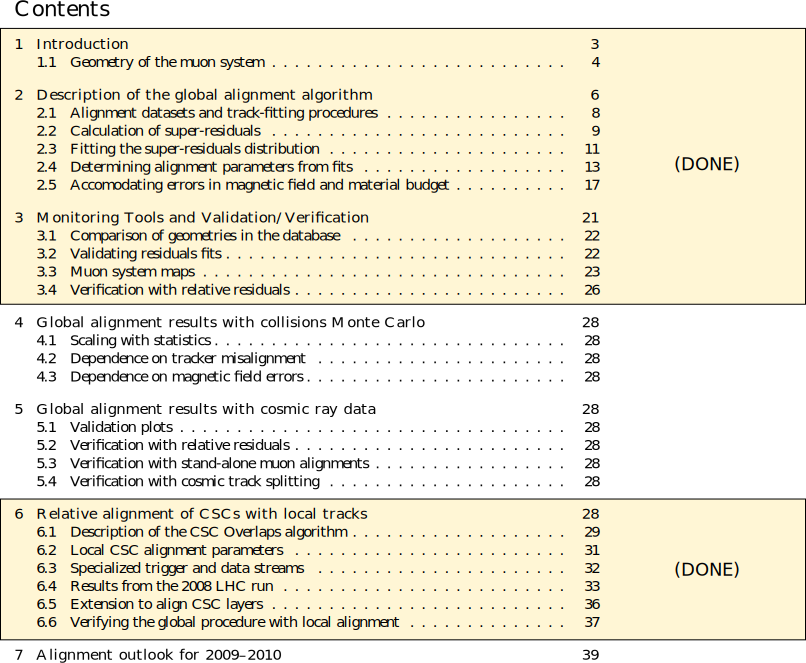
\includegraphics[width=0.9\linewidth]{contents.pdf}
\end{frame}

\begin{frame}
\frametitle{Alignment procedure in brief}

\begin{itemize}
\item Fit tracks to tracker, propagate into muon system
\item Collect residuals with respect to tracks in two bins: $\mu^+$ and $\mu^-$
\item Fit residuals to theoretical curve, accounting for
\begin{itemize}
\item correlations that yield alignments: $\phi_z$ and local $z$
\item other significant correlations that may distort the shape
\end{itemize}

\vspace{0.25 cm}
\begin{columns}
\column{0.5\linewidth}
\includegraphics[width=\linewidth]{phiz_diagram.pdf}
\column{0.35\linewidth}
\includegraphics[width=\linewidth]{zpos_diagram.pdf}
\end{columns}

\vspace{0.25 cm}
\item Average the fit results from the two bins and update geometry
\item Iterate if necessary
\begin{itemize}
\item in principle, iteration is not necessary because track-fitting is independent of alignment
\item if imperfectly modeled by fit function, correlations between parameters (especially angles) can be resolved by iteration
\end{itemize}
\end{itemize}
\end{frame}

\begin{frame}
\frametitle{Summary of fitting methods}
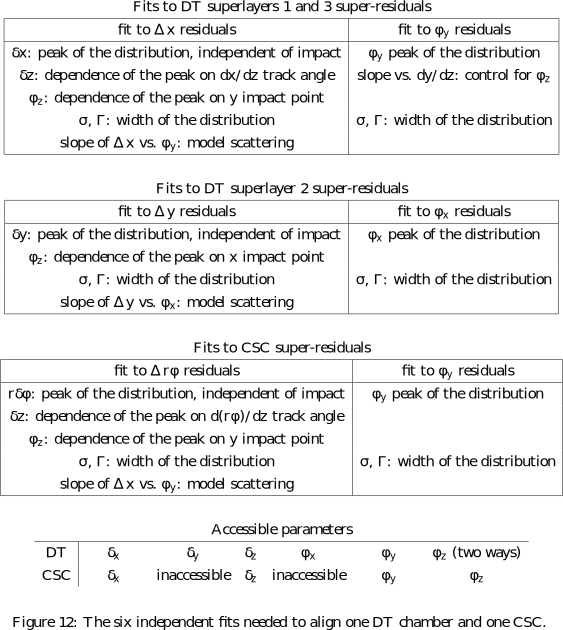
\includegraphics[width=0.7\linewidth]{parameter_fits.pdf}
\end{frame}

\begin{frame}
\frametitle{Sample fits 1/3 (MC)}

Two independent fits: $\mu^+$ in top row, $\mu^-$ in bottom row

\vfill
Lines are crest of peak function in different projections

\vfill
Vertical line on bell curve is average of $\mu^+$ and $\mu^-$

\vfill
\includegraphics[height=\linewidth, angle=90]{exampleDT_rphi.pdf}
\end{frame}

\begin{frame}
\frametitle{Sample fits 2/3 (MC)}

Superlayer 2 fit is independent of superlayer~1\&3

\vfill
Can cross-check $\phi_z$ and local $z$ measurements (opposite sign convention)

\vfill
But lower precision (local $z$ is held fixed in this example)

\vfill
\includegraphics[height=\linewidth, angle=90]{exampleDT_z.pdf}
\end{frame}

\begin{frame}
\frametitle{Sample fits 3/3 (MC)}

\mbox{ } \hfill \includegraphics[width=0.8\linewidth]{strip_direction.pdf} \hfill \mbox{ }

\vfill
CSCs included in the same way, except that correction is in
curvilinear $r\phi$, rather than cartesian local $x$

\vfill
\includegraphics[height=\linewidth, angle=90]{exampleCSC_rphi.pdf}
\end{frame}

\begin{frame}
\frametitle{New residuals maps 1/3 (MC)}

Best DT station (1) and wheel (0) with 50~pb$^{-1}$

\vfill
No tracker misalignment included yet

\vfill
\includegraphics[height=\linewidth, angle=90]{examplemap_rphi1.pdf}
\end{frame}

\begin{frame}
\frametitle{New residuals maps 2/3 (MC)}

Worst DT station (4) and wheel ($\pm$2), same $\displaystyle \int \mathcal{L} \, dt$

\vfill
\includegraphics[height=\linewidth, angle=90]{examplemap_rphi4.pdf}
\end{frame}

\begin{frame}
\frametitle{New residuals maps 3/3 (MC)}

CSC plots are vs.\ $\phi$ and vs.\ $R$ (ME$+$1/1a, 1/1b, 1/2, 1/3 below)

\vfill
\includegraphics[height=\linewidth, angle=90]{examplemap_CSCrphi1.pdf}
\end{frame}

\begin{frame}
\frametitle{Full CSC Overlaps write-up}

Method and 2008 results in complete detail (11 pages), polished and final

\vfill
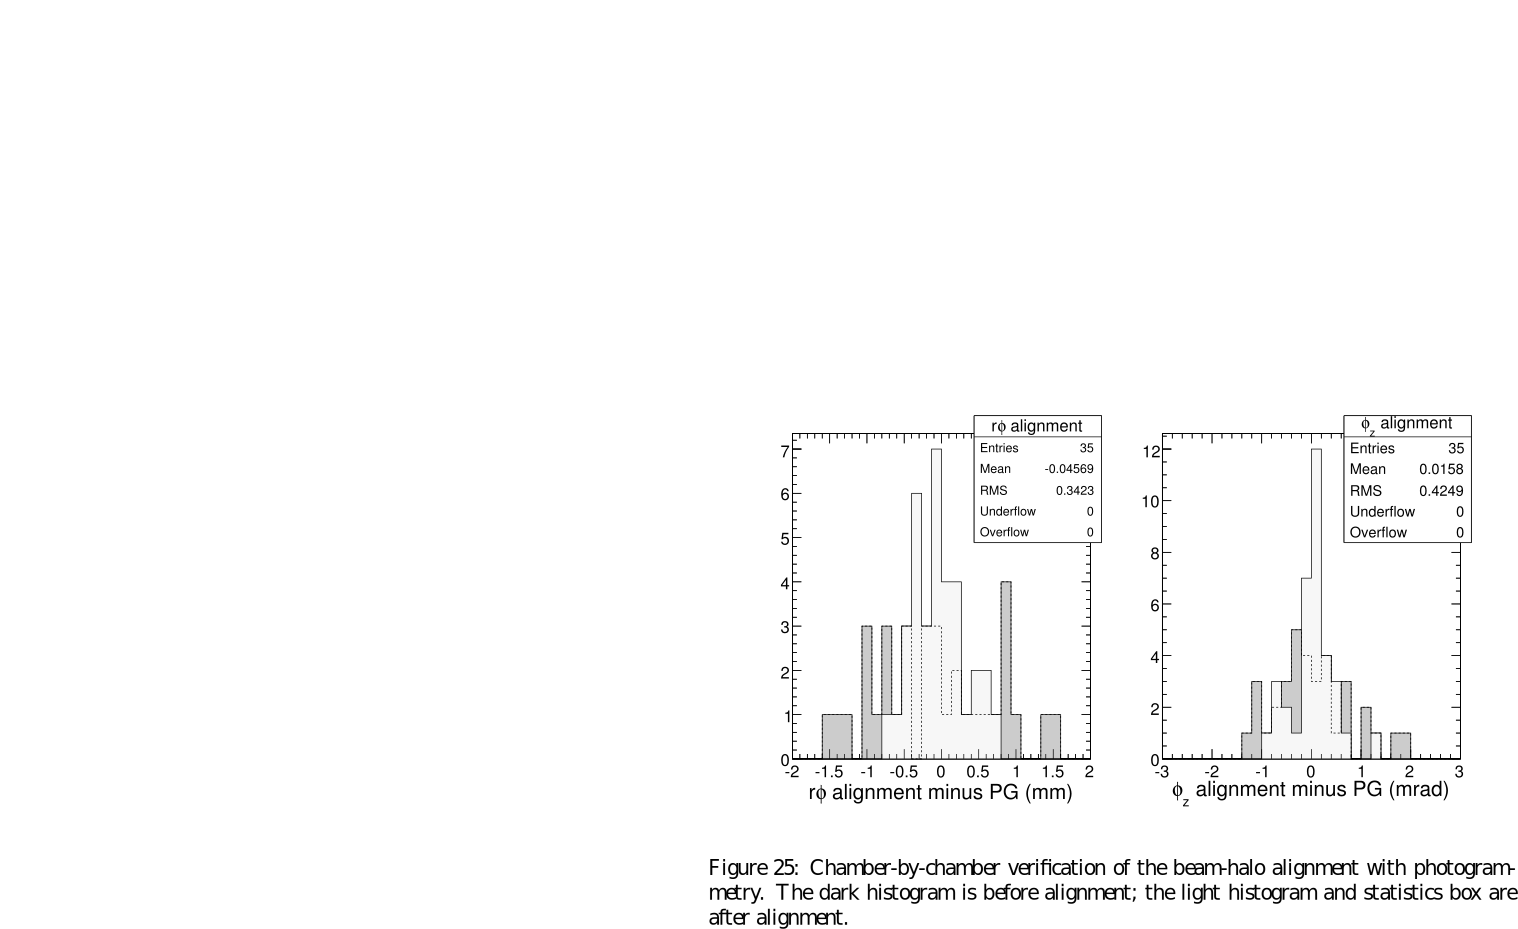
\includegraphics[width=\linewidth]{CSCoverlaps_writeup.pdf}
\end{frame}

\begin{frame}
\frametitle{Plots from CRAFT data}

\begin{columns}
\column{0.65\linewidth}

\includegraphics[height=\linewidth, angle=90]{example_zpos_m1_1_4.pdf}

\includegraphics[height=\linewidth, angle=90]{example_zpos_map_1_4.pdf}

\column{0.4\linewidth}
\begin{itemize}\setlength{\itemsep}{0.25 cm}
\item Observations of radial misalignments in highest-statistics chambers
\item Radial corrections restricted to zero in this example
\item Statistically significant in some chambers, not in others
\end{itemize}
\end{columns}
\end{frame}

\begin{frame}
\frametitle{Sawtooth still present}

\begin{columns}
\column{0.65\linewidth}

\includegraphics[height=\linewidth, angle=90]{sawtooth_still_present.pdf}

\includegraphics[height=\linewidth, angle=90]{sawtooth_also_in_phiy.pdf}

\column{0.4\linewidth}
\begin{itemize}\setlength{\itemsep}{0.25 cm}
\item ``Sawtooth'' is unexplained \mbox{$r\phi$ residual vs.\ $\phi$} slopes within chambers
\item Also present in \mbox{$\phi_y$ residuals vs.\ $\phi$} (expected from single-chamber studies)
\item Full presentation of single-chamber studies in April~2 DT-DPG
\end{itemize}
\end{columns}
\end{frame}

\begin{frame}
\frametitle{Angular alignment corrections}

\begin{columns}
\column{0.5\linewidth}

Largest $\phi_y$ example I could find with high statistics: $3.86 \pm 0.06$~mrad

\vspace{0.1 cm}
\includegraphics[height=\linewidth, angle=90]{large_phiy_corrections.pdf}

\vspace{0.25 cm}
Largest $\phi_x$ example I could find with high statistics: $-1.17 \pm 0.11$~mrad

\vspace{0.1 cm}
\includegraphics[height=\linewidth, angle=90]{no_significant_phix_corrections.pdf}

\column{0.4\linewidth}
\begin{itemize}\setlength{\itemsep}{0.25 cm}
\item $\phi_y$ measured with track-segment angle differences (see note for ``super-residuals'')
\begin{itemize}
\item some are significant and large: few mrad
\end{itemize}

\item $\phi_x$: same technique with superlayer 2
\begin{itemize}
\item generally small and/or \mbox{low resolution\hspace{-1 cm}}
\end{itemize}

\item Vertical line is again $\mu^+$/$\mu^-$ average

\end{itemize}
\end{columns}
\end{frame}

\begin{frame}
\frametitle{What will be for sign-off?}
\begin{itemize}\setlength{\itemsep}{0.3 cm}
\item We'll be signing off the procedure as described in the note
\begin{itemize}
\item already presented in final, digestable form
\end{itemize}
\item Sign-offable {\it constants} will require some tweaks:
\begin{itemize}\setlength{\itemsep}{0.15 cm}
\item need to decide which parameters to align for which chambers
\item how many iterations are sufficient (to work out couplings between parameters)
\item in what order (some parameter dependencies are one-way)

for example, CSC Overlaps was optimized by $\phi_y \to x \to \phi_z$
\end{itemize}
\item Final constants for tracker-pointing re-processing will need to
  be generated with new tracker alignment, when it becomes available
\end{itemize}
\end{frame}

%% \section*{First section}
%% \begin{frame}
%% \begin{center}
%% \Huge \textcolor{blue}{First section}
%% \end{center}
%% \end{frame}

\begin{frame}
\frametitle{Conclusions}
\begin{itemize}\setlength{\itemsep}{0.4 cm}
\item Read the note!  What is written is in final or nearly-final form
\begin{itemize}
\item this is the detailed CMS Note that will back up a shorter publication, to be written (by abridgement)
\end{itemize}
\item It includes everything about the CSC Overlaps procedure and results
\item We can now align globalMuon-accessible DTs in any of 6 d.o.f.\ with highly descriptive residuals fits
\begin{itemize}\setlength{\itemsep}{0.2 cm}
\item 6~mm radial misalignments observed
\item 4~mrad $\phi_y$ rotations observed (important for $q$ and $p_T$)
\item most $\phi_x$ are small or consistent with zero
\end{itemize}
\item Basic procedure established; working on details of iteration strategy
\item Documentation is kept in sync with results
\end{itemize}
\label{numpages}
\end{frame}

\end{document}
